\documentclass[11pt, a4paper]{article}\usepackage[]{graphicx}\usepackage[]{xcolor}
% maxwidth is the original width if it is less than linewidth
% otherwise use linewidth (to make sure the graphics do not exceed the margin)
\makeatletter
\def\maxwidth{ %
  \ifdim\Gin@nat@width>\linewidth
    \linewidth
  \else
    \Gin@nat@width
  \fi
}
\makeatother

\definecolor{fgcolor}{rgb}{0.345, 0.345, 0.345}
\newcommand{\hlnum}[1]{\textcolor[rgb]{0.686,0.059,0.569}{#1}}%
\newcommand{\hlstr}[1]{\textcolor[rgb]{0.192,0.494,0.8}{#1}}%
\newcommand{\hlcom}[1]{\textcolor[rgb]{0.678,0.584,0.686}{\textit{#1}}}%
\newcommand{\hlopt}[1]{\textcolor[rgb]{0,0,0}{#1}}%
\newcommand{\hlstd}[1]{\textcolor[rgb]{0.345,0.345,0.345}{#1}}%
\newcommand{\hlkwa}[1]{\textcolor[rgb]{0.161,0.373,0.58}{\textbf{#1}}}%
\newcommand{\hlkwb}[1]{\textcolor[rgb]{0.69,0.353,0.396}{#1}}%
\newcommand{\hlkwc}[1]{\textcolor[rgb]{0.333,0.667,0.333}{#1}}%
\newcommand{\hlkwd}[1]{\textcolor[rgb]{0.737,0.353,0.396}{\textbf{#1}}}%
\let\hlipl\hlkwb

\usepackage{framed}
\makeatletter
\newenvironment{kframe}{%
 \def\at@end@of@kframe{}%
 \ifinner\ifhmode%
  \def\at@end@of@kframe{\end{minipage}}%
  \begin{minipage}{\columnwidth}%
 \fi\fi%
 \def\FrameCommand##1{\hskip\@totalleftmargin \hskip-\fboxsep
 \colorbox{shadecolor}{##1}\hskip-\fboxsep
     % There is no \\@totalrightmargin, so:
     \hskip-\linewidth \hskip-\@totalleftmargin \hskip\columnwidth}%
 \MakeFramed {\advance\hsize-\width
   \@totalleftmargin\z@ \linewidth\hsize
   \@setminipage}}%
 {\par\unskip\endMakeFramed%
 \at@end@of@kframe}
\makeatother

\definecolor{shadecolor}{rgb}{.97, .97, .97}
\definecolor{messagecolor}{rgb}{0, 0, 0}
\definecolor{warningcolor}{rgb}{1, 0, 1}
\definecolor{errorcolor}{rgb}{1, 0, 0}
\newenvironment{knitrout}{}{} % an empty environment to be redefined in TeX

\usepackage{alltt}

\usepackage[top=1 in, bottom = 1 in, left = 1 in, right = 1 in ]{geometry}

\usepackage{amsmath, amssymb, amsfonts}
\usepackage{enumerate}

\title{One-way ANOVA - Fixed Effects Model}
\author{Ananda Biswas}
\date{}
\IfFileExists{upquote.sty}{\usepackage{upquote}}{}
\begin{document}

\maketitle



\begin{knitrout}
\definecolor{shadecolor}{rgb}{0.969, 0.969, 0.969}\color{fgcolor}\begin{kframe}
\begin{alltt}
\hlstd{life_hours} \hlkwb{<-} \hlkwd{read.csv}\hlstd{(}\hlstr{"D:\textbackslash{}\textbackslash{}data_sets\textbackslash{}\textbackslash{}life_hours_of_bulbs_data.csv"}\hlstd{,}
    \hlkwc{stringsAsFactors} \hlstd{=} \hlnum{TRUE}\hlstd{)}
\end{alltt}
\end{kframe}
\end{knitrout}

\begin{knitrout}
\definecolor{shadecolor}{rgb}{0.969, 0.969, 0.969}\color{fgcolor}\begin{kframe}
\begin{alltt}
\hlstd{life_hours}
\end{alltt}
\begin{verbatim}
##    batch life_of_bulb
## 1      A         1600
## 2      A         1610
## 3      A         1650
## 4      A         1680
## 5      A         1700
## 6      A         1720
## 7      A         1800
## 8      B         1580
## 9      B         1640
## 10     B         1640
## 11     B         1700
## 12     B         1750
## 13     C         1460
## 14     C         1550
## 15     C         1600
## 16     C         1620
## 17     C         1640
## 18     C         1660
## 19     C         1740
## 20     C         1820
## 21     D         1510
## 22     D         1520
## 23     D         1530
## 24     D         1570
## 25     D         1600
## 26     D         1680
\end{verbatim}
\end{kframe}
\end{knitrout}

\begin{knitrout}
\definecolor{shadecolor}{rgb}{0.969, 0.969, 0.969}\color{fgcolor}\begin{kframe}
\begin{alltt}
\hlkwd{dim}\hlstd{(life_hours)}
\end{alltt}
\begin{verbatim}
## [1] 26  2
\end{verbatim}
\end{kframe}
\end{knitrout}

\begin{knitrout}
\definecolor{shadecolor}{rgb}{0.969, 0.969, 0.969}\color{fgcolor}\begin{kframe}
\begin{alltt}
\hlkwd{names}\hlstd{(life_hours)}
\end{alltt}
\begin{verbatim}
## [1] "batch"        "life_of_bulb"
\end{verbatim}
\end{kframe}
\end{knitrout}

\begin{knitrout}
\definecolor{shadecolor}{rgb}{0.969, 0.969, 0.969}\color{fgcolor}\begin{kframe}
\begin{alltt}
\hlkwd{head}\hlstd{(life_hours)}
\end{alltt}
\begin{verbatim}
##   batch life_of_bulb
## 1     A         1600
## 2     A         1610
## 3     A         1650
## 4     A         1680
## 5     A         1700
## 6     A         1720
\end{verbatim}
\end{kframe}
\end{knitrout}

\begin{knitrout}
\definecolor{shadecolor}{rgb}{0.969, 0.969, 0.969}\color{fgcolor}\begin{kframe}
\begin{alltt}
\hlkwd{tail}\hlstd{(life_hours)}
\end{alltt}
\begin{verbatim}
##    batch life_of_bulb
## 21     D         1510
## 22     D         1520
## 23     D         1530
## 24     D         1570
## 25     D         1600
## 26     D         1680
\end{verbatim}
\end{kframe}
\end{knitrout}


\begin{knitrout}
\definecolor{shadecolor}{rgb}{0.969, 0.969, 0.969}\color{fgcolor}\begin{kframe}
\begin{alltt}
\hlkwd{summary}\hlstd{(life_hours)}
\end{alltt}
\begin{verbatim}
##  batch  life_of_bulb 
##  A:7   Min.   :1460  
##  B:5   1st Qu.:1585  
##  C:8   Median :1640  
##  D:6   Mean   :1637  
##        3rd Qu.:1695  
##        Max.   :1820
\end{verbatim}
\end{kframe}
\end{knitrout}

\newpage

\begin{knitrout}
\definecolor{shadecolor}{rgb}{0.969, 0.969, 0.969}\color{fgcolor}\begin{kframe}
\begin{alltt}
\hlkwd{library}\hlstd{(tidyverse)}
\end{alltt}


{\ttfamily\noindent\color{warningcolor}{\#\# Warning: package 'tidyverse' was built under R version 4.2.3}}

{\ttfamily\noindent\color{warningcolor}{\#\# Warning: package 'ggplot2' was built under R version 4.2.2}}

{\ttfamily\noindent\color{warningcolor}{\#\# Warning: package 'tibble' was built under R version 4.2.3}}

{\ttfamily\noindent\color{warningcolor}{\#\# Warning: package 'tidyr' was built under R version 4.2.3}}

{\ttfamily\noindent\color{warningcolor}{\#\# Warning: package 'readr' was built under R version 4.2.2}}

{\ttfamily\noindent\color{warningcolor}{\#\# Warning: package 'purrr' was built under R version 4.2.3}}

{\ttfamily\noindent\color{warningcolor}{\#\# Warning: package 'dplyr' was built under R version 4.2.3}}

{\ttfamily\noindent\color{warningcolor}{\#\# Warning: package 'stringr' was built under R version 4.2.3}}

{\ttfamily\noindent\color{warningcolor}{\#\# Warning: package 'forcats' was built under R version 4.2.2}}

{\ttfamily\noindent\color{warningcolor}{\#\# Warning: package 'lubridate' was built under R version 4.2.2}}

{\ttfamily\noindent\itshape\color{messagecolor}{\#\# -- Attaching core tidyverse packages ------------------------ tidyverse 2.0.0 --\\\#\# v dplyr \ \ \ \ 1.1.3 \ \ \ \ v readr \ \ \ \ 2.1.4\\\#\# v forcats \ \ 1.0.0 \ \ \ \ v stringr \ \ 1.5.0\\\#\# v ggplot2 \ \ 3.4.1 \ \ \ \ v tibble \ \ \ 3.2.1\\\#\# v lubridate 1.9.2 \ \ \ \ v tidyr \ \ \ \ 1.3.0\\\#\# v purrr \ \ \ \ 1.0.2 \ \ \ \ \\\#\# -- Conflicts ------------------------------------------ tidyverse\_conflicts() --\\\#\# x dplyr::filter() masks stats::filter()\\\#\# x dplyr::lag() \ \ \ masks stats::lag()\\\#\# i Use the conflicted package (<http://conflicted.r-lib.org/>) to force all conflicts to become errors}}\end{kframe}
\end{knitrout}

\newpage

\begin{knitrout}
\definecolor{shadecolor}{rgb}{0.969, 0.969, 0.969}\color{fgcolor}\begin{kframe}
\begin{alltt}
\hlstd{life_hours} \hlopt
    \hlkwd{ggplot}\hlstd{(}\hlkwd{aes}\hlstd{(}\hlkwc{x} \hlstd{= batch,} \hlkwc{y} \hlstd{= life_of_bulb))} \hlopt{+} \hlkwd{stat_boxplot}\hlstd{(}\hlkwc{geom} \hlstd{=} \hlstr{"errorbar"}\hlstd{,}
    \hlkwc{linewidth} \hlstd{=} \hlnum{1}\hlstd{)} \hlopt{+} \hlkwd{geom_boxplot}\hlstd{(}\hlkwc{fill} \hlstd{=} \hlstr{"#21F731"}\hlstd{)} \hlopt{+}
    \hlkwd{labs}\hlstd{(}\hlkwc{x} \hlstd{=} \hlstr{"Batch"}\hlstd{,} \hlkwc{y} \hlstd{=} \hlstr{"Life-hours of Bulb"}\hlstd{,} \hlkwc{title} \hlstd{=} \hlstr{"Life-hours of Bulbs vs Batches"}\hlstd{)}
\end{alltt}
\end{kframe}
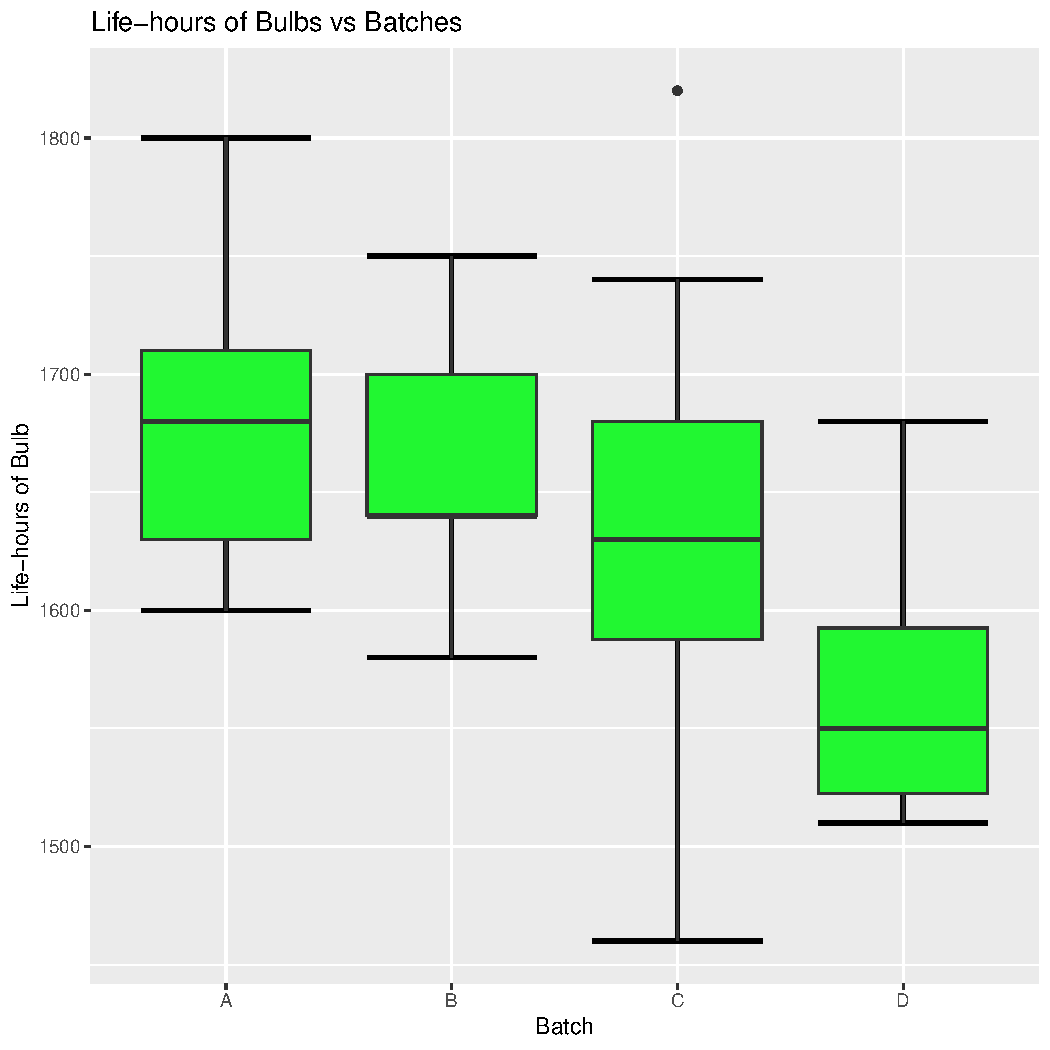
\includegraphics[width=\maxwidth]{figure/unnamed-chunk-9-1} 
\end{knitrout}


\newpage

$\bullet$ \textbf{Testing Normality of Our Sample}

\begin{knitrout}
\definecolor{shadecolor}{rgb}{0.969, 0.969, 0.969}\color{fgcolor}\begin{kframe}
\begin{alltt}
\hlstd{life_hours} \hlopt
    \hlkwd{ggplot}\hlstd{(}\hlkwd{aes}\hlstd{(}\hlkwc{sample} \hlstd{= life_of_bulb))} \hlopt{+} \hlkwd{geom_qq}\hlstd{(}\hlkwc{size} \hlstd{=} \hlnum{2}\hlstd{,}
    \hlkwc{col} \hlstd{=} \hlstr{"blue"}\hlstd{)} \hlopt{+} \hlkwd{geom_qq_line}\hlstd{(}\hlkwc{col} \hlstd{=} \hlstr{"red"}\hlstd{,} \hlkwc{linewidth} \hlstd{=} \hlnum{1}\hlstd{)} \hlopt{+}
    \hlkwd{labs}\hlstd{(}\hlkwc{x} \hlstd{=} \hlstr{"Theoretical Quantiles"}\hlstd{,} \hlkwc{y} \hlstd{=} \hlstr{"Sample Quantiles"}\hlstd{,}
        \hlkwc{title} \hlstd{=} \hlstr{"Normal Q-Q Plot"}\hlstd{)}
\end{alltt}
\end{kframe}
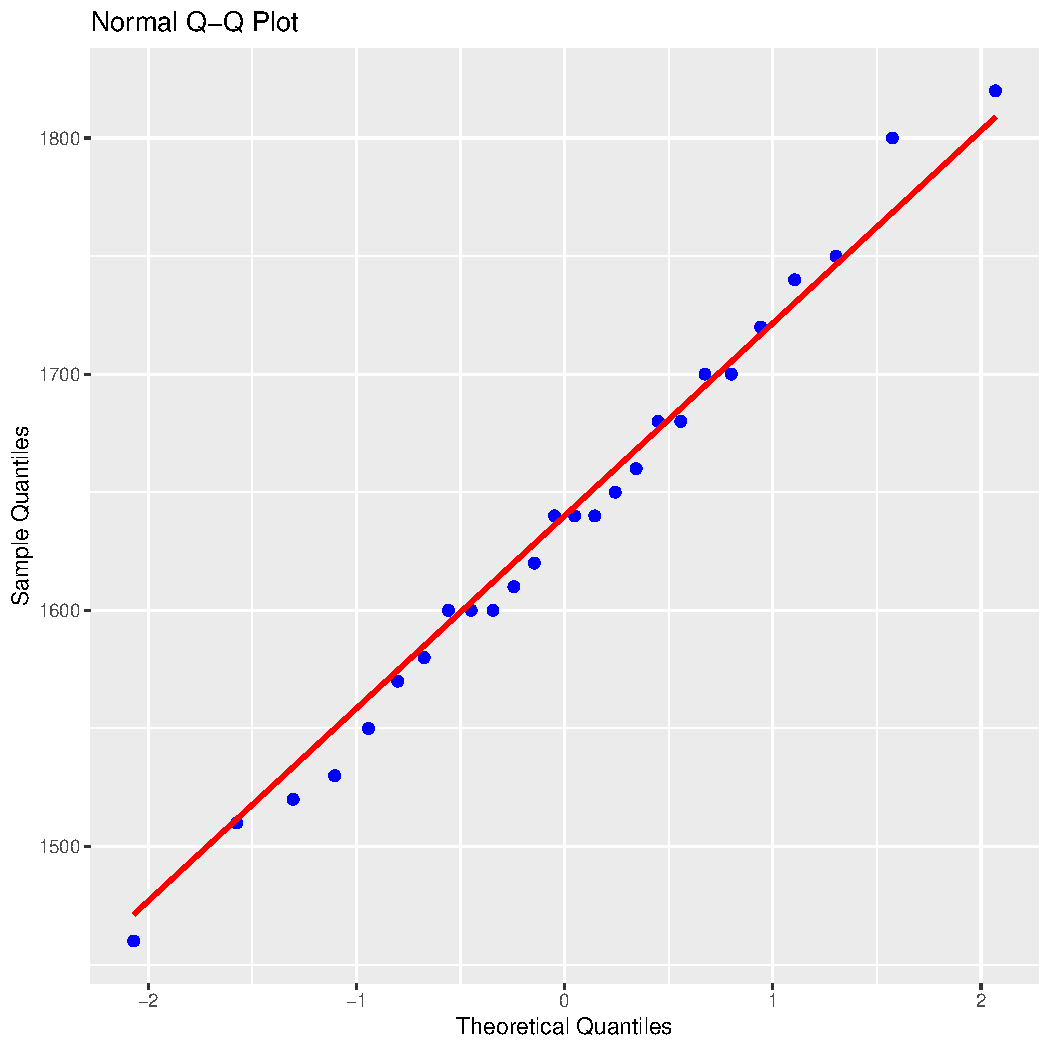
\includegraphics[width=\maxwidth]{figure/unnamed-chunk-10-1} 
\end{knitrout}

We see that the line is a good fit. Hence, we conclude the sample is from a normal population.


\newpage

$\bullet$ \textbf{Testing Equality of Several Population Variances (Homogenity)}

\begin{knitrout}
\definecolor{shadecolor}{rgb}{0.969, 0.969, 0.969}\color{fgcolor}\begin{kframe}
\begin{alltt}
\hlstd{homo_test} \hlkwb{<-} \hlkwd{bartlett.test}\hlstd{(life_of_bulb} \hlopt{~} \hlstd{batch,} \hlkwc{data} \hlstd{= life_hours)}
\hlstd{homo_test}
\end{alltt}
\begin{verbatim}
## 
## 	Bartlett test of homogeneity of variances
## 
## data:  life_of_bulb by batch
## Bartlett's K-squared = 2.508, df = 3, p-value = 0.4738
\end{verbatim}
\end{kframe}
\end{knitrout}

\begin{figure}[h]
\centering
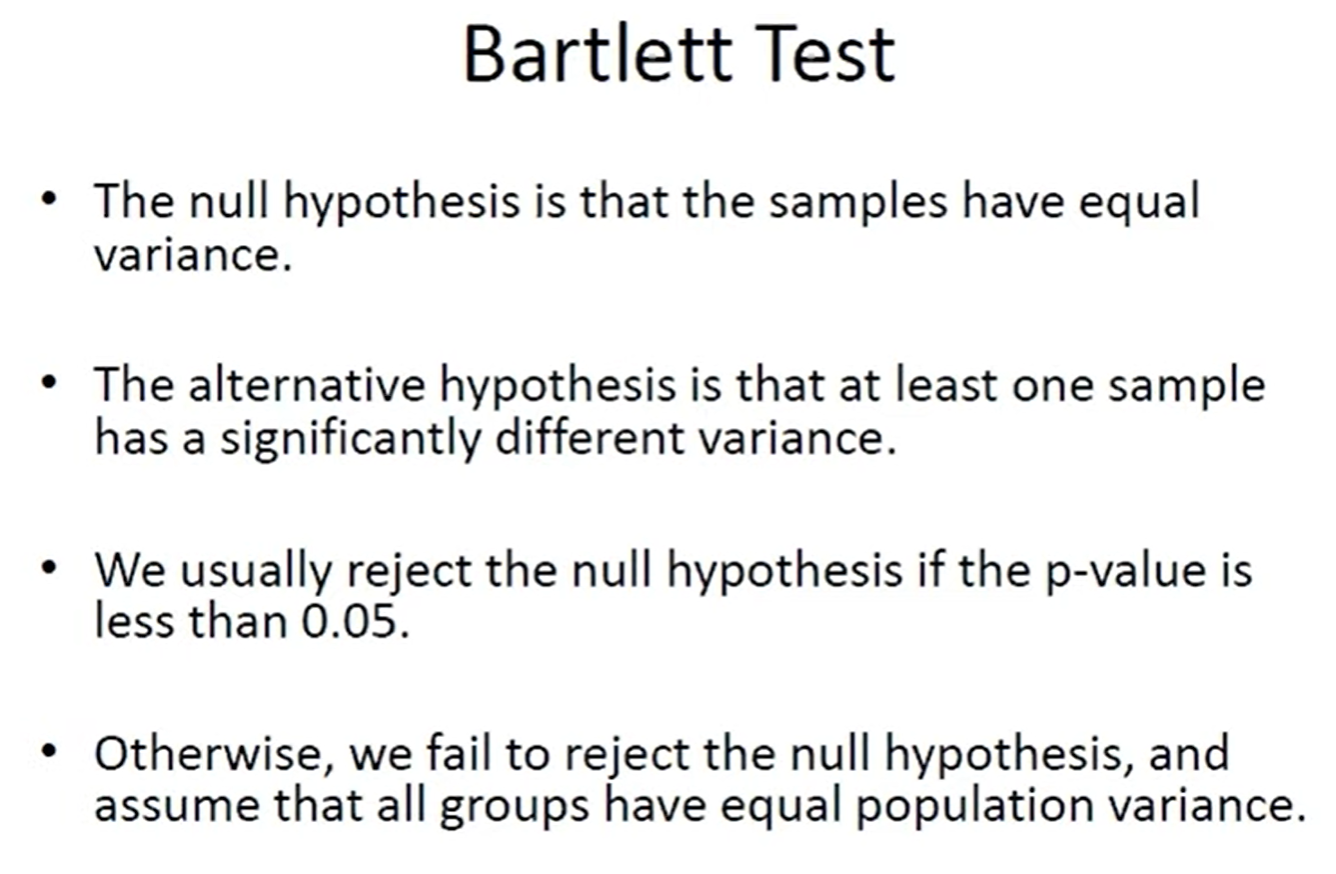
\includegraphics[scale = 0.5]{bartlett's_test}\\
\end{figure}
	
\begin{knitrout}
\definecolor{shadecolor}{rgb}{0.969, 0.969, 0.969}\color{fgcolor}\begin{kframe}
\begin{alltt}
\hlstd{homo_test}\hlopt{$}\hlstd{p.value}
\end{alltt}
\begin{verbatim}
## [1] 0.4738465
\end{verbatim}
\end{kframe}
\end{knitrout}

See that the p-value is much higher than $\alpha = 0.05$, so we fail to reject the null hypothesis and conclude that our homoscedastic assumption is true.

\newpage

\begin{knitrout}
\definecolor{shadecolor}{rgb}{0.969, 0.969, 0.969}\color{fgcolor}\begin{kframe}
\begin{alltt}
\hlstd{fit1} \hlkwb{<-} \hlkwd{lm}\hlstd{(life_of_bulb} \hlopt{~} \hlstd{batch,} \hlkwc{data} \hlstd{= life_hours)}
\hlkwd{summary}\hlstd{(fit1)}
\end{alltt}
\begin{verbatim}
## 
## Call:
## lm(formula = life_of_bulb ~ batch, data = life_hours)
## 
## Residuals:
##      Min       1Q   Median       3Q      Max 
## -176.250  -45.833   -8.125   36.417  183.750 
## 
## Coefficients:
##             Estimate Std. Error t value Pr(>|t|)    
## (Intercept)  1680.00      31.35  53.589   <2e-16 ***
## batchB        -18.00      48.57  -0.371   0.7145    
## batchC        -43.75      42.93  -1.019   0.3192    
## batchD       -111.67      46.15  -2.420   0.0242 *  
## ---
## Signif. codes:  0 '***' 0.001 '**' 0.01 '*' 0.05 '.' 0.1 ' ' 1
## 
## Residual standard error: 82.94 on 22 degrees of freedom
## Multiple R-squared:  0.2267,	Adjusted R-squared:  0.1212 
## F-statistic: 2.149 on 3 and 22 DF,  p-value: 0.1229
\end{verbatim}
\end{kframe}
\end{knitrout}

\begin{knitrout}
\definecolor{shadecolor}{rgb}{0.969, 0.969, 0.969}\color{fgcolor}\begin{kframe}
\begin{alltt}
\hlkwd{model.matrix}\hlstd{(fit1)}
\end{alltt}
\begin{verbatim}
##    (Intercept) batchB batchC batchD
## 1            1      0      0      0
## 2            1      0      0      0
## 3            1      0      0      0
## 4            1      0      0      0
## 5            1      0      0      0
## 6            1      0      0      0
## 7            1      0      0      0
## 8            1      1      0      0
## 9            1      1      0      0
## 10           1      1      0      0
## 11           1      1      0      0
## 12           1      1      0      0
## 13           1      0      1      0
## 14           1      0      1      0
## 15           1      0      1      0
## 16           1      0      1      0
## 17           1      0      1      0
## 18           1      0      1      0
## 19           1      0      1      0
## 20           1      0      1      0
## 21           1      0      0      1
## 22           1      0      0      1
## 23           1      0      0      1
## 24           1      0      0      1
## 25           1      0      0      1
## 26           1      0      0      1
## attr(,"assign")
## [1] 0 1 1 1
## attr(,"contrasts")
## attr(,"contrasts")$batch
## [1] "contr.treatment"
\end{verbatim}
\end{kframe}
\end{knitrout}

\begin{knitrout}
\definecolor{shadecolor}{rgb}{0.969, 0.969, 0.969}\color{fgcolor}\begin{kframe}
\begin{alltt}
\hlstd{fit1}\hlopt{$}\hlstd{rank}
\end{alltt}
\begin{verbatim}
## [1] 4
\end{verbatim}
\end{kframe}
\end{knitrout}

As the rank of the model matrix is 4, only 4 parameters have been estimated. \textit{batchA} or $\alpha_1$ has been forced 0.

\newpage

\begin{knitrout}
\definecolor{shadecolor}{rgb}{0.969, 0.969, 0.969}\color{fgcolor}\begin{kframe}
\begin{alltt}
\hlstd{life_hours_anova} \hlkwb{<-} \hlkwd{aov}\hlstd{(life_of_bulb} \hlopt{~} \hlstd{batch,} \hlkwc{data} \hlstd{= life_hours)}
\hlkwd{summary}\hlstd{(life_hours_anova)}
\end{alltt}
\begin{verbatim}
##             Df Sum Sq Mean Sq F value Pr(>F)
## batch        3  44361   14787   2.149  0.123
## Residuals   22 151351    6880
\end{verbatim}
\end{kframe}
\end{knitrout}

See that, p-value corresponding to the test of equality of batch means is 0.123 which is much higher than $\alpha = 0.05$. So, we conclude that there is no significant difference between the batch means.


\newpage

$\bullet$ \textbf{Pairwise Comparison}(although not necessary here)
\begin{knitrout}
\definecolor{shadecolor}{rgb}{0.969, 0.969, 0.969}\color{fgcolor}\begin{kframe}
\begin{alltt}
\hlkwd{TukeyHSD}\hlstd{(life_hours_anova)}
\end{alltt}
\begin{verbatim}
##   Tukey multiple comparisons of means
##     95% family-wise confidence level
## 
## Fit: aov(formula = life_of_bulb ~ batch, data = life_hours)
## 
## $batch
##           diff       lwr       upr     p adj
## B-A  -18.00000 -152.8615 116.86146 0.9821643
## C-A  -43.75000 -162.9518  75.45182 0.7401446
## D-A -111.66667 -239.8048  16.47143 0.1025335
## C-B  -25.75000 -157.0525 105.55248 0.9470311
## D-B  -93.66667 -233.1322  45.79889 0.2714523
## D-C  -67.91667 -192.3036  56.47024 0.4452307
\end{verbatim}
\end{kframe}
\end{knitrout}

See that, all the p-values are greater than 0.05, implying that no two of the batch means differ significantly.

\newpage

\begin{knitrout}
\definecolor{shadecolor}{rgb}{0.969, 0.969, 0.969}\color{fgcolor}\begin{kframe}
\begin{alltt}
\hlstd{df1} \hlkwb{<-} \hlkwd{data.frame}\hlstd{(}\hlkwc{batch} \hlstd{= life_hours}\hlopt{$}\hlstd{batch,} \hlkwc{residuals} \hlstd{= fit1}\hlopt{$}\hlstd{residuals)}
\end{alltt}
\end{kframe}
\end{knitrout}

\begin{knitrout}
\definecolor{shadecolor}{rgb}{0.969, 0.969, 0.969}\color{fgcolor}\begin{kframe}
\begin{alltt}
\hlstd{df1} \hlopt
    \hlkwd{ggplot}\hlstd{(}\hlkwd{aes}\hlstd{(}\hlkwc{x} \hlstd{= batch,} \hlkwc{y} \hlstd{= residuals))} \hlopt{+} \hlkwd{geom_hline}\hlstd{(}\hlkwc{yintercept} \hlstd{=} \hlnum{0}\hlstd{,}
    \hlkwc{col} \hlstd{=} \hlstr{"#FB2209"}\hlstd{,} \hlkwc{linewidth} \hlstd{=} \hlnum{1}\hlstd{)} \hlopt{+} \hlkwd{stat_boxplot}\hlstd{(}\hlkwc{geom} \hlstd{=} \hlstr{"errorbar"}\hlstd{,}
    \hlkwc{linewidth} \hlstd{=} \hlnum{1}\hlstd{)} \hlopt{+} \hlkwd{geom_boxplot}\hlstd{(}\hlkwc{fill} \hlstd{=} \hlstr{"#F10BCB"}\hlstd{)} \hlopt{+}
    \hlkwd{labs}\hlstd{(}\hlkwc{x} \hlstd{=} \hlstr{"Sample"}\hlstd{,} \hlkwc{y} \hlstd{=} \hlstr{"Residuals"}\hlstd{,} \hlkwc{title} \hlstd{=} \hlstr{"Residual Plot"}\hlstd{)}
\end{alltt}
\end{kframe}
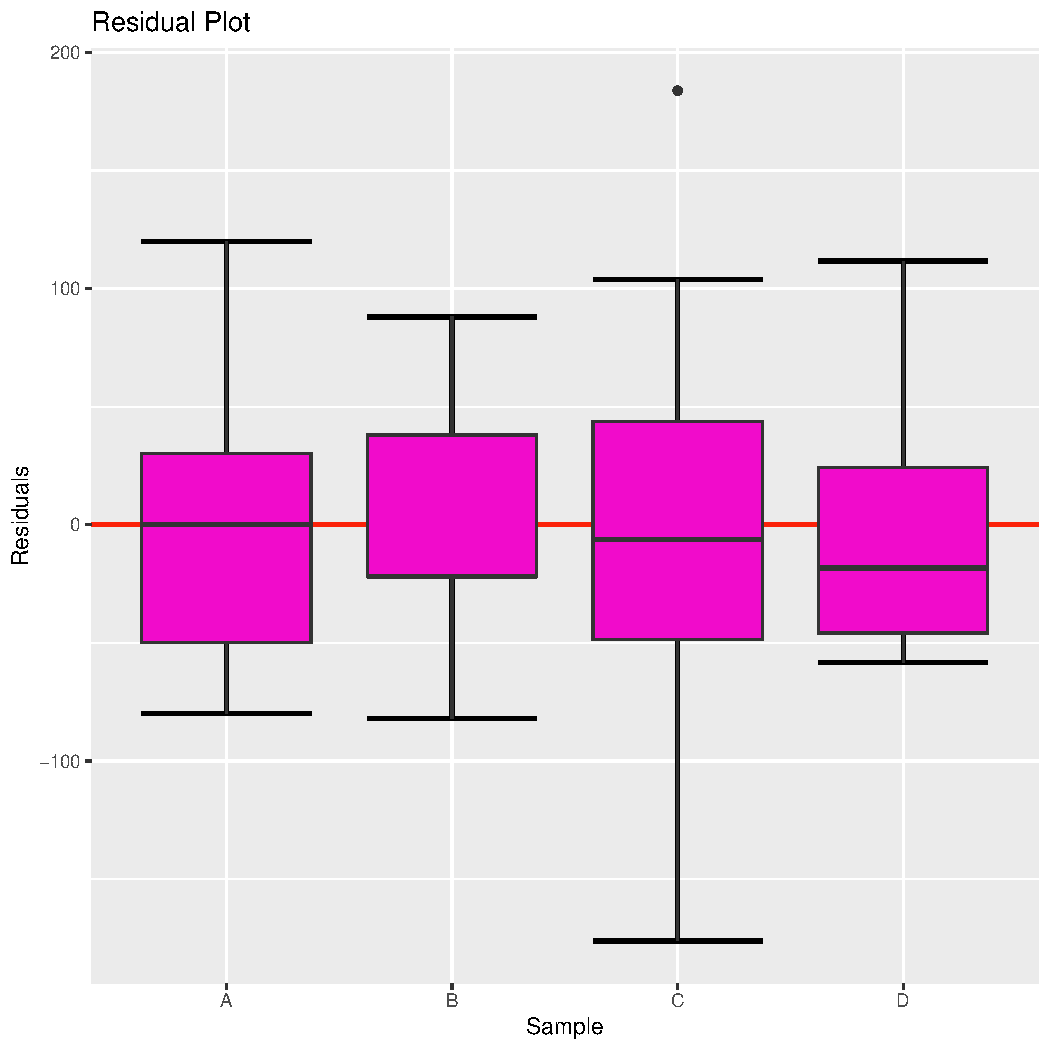
\includegraphics[width=\maxwidth]{figure/unnamed-chunk-19-1} 
\end{knitrout}


\end{document}
